\section{Supplemental Results}\label{a:res}
%===================================================================================================
\subsection{Base Case}\label{a:res.bc}
%---------------------------------------------------------------------------------------------------
\subsubsection{Distribution of Infections}\label{a:res.bc.inf}
The following figures explore the numbers and proportions of infections
transmitted between risk groups, stratified by partnership type throughout the epidemic.
For each stratification (from, to, partnership type, and year),
we use the median numbers of infections across all model fits.
Figure~\ref{fig:inf.part} illustrates
infections transmitted via the modelled partnership types over time in the base case, while
Figure~\ref{fig:inf.frto} illustrates
the risk groups transmitting (\subref{fig:inf.fr}) and acquiring (\subref{fig:inf.to}) infections.
Figure~\ref{fig:inf.alluvial} illustrates the distribution of infections
stratified by all three factors every 10 years using an alluvial diagram.
Figure~\ref{fig:inf.ratio} illustrates
the ratio of infections transmitted from vs acquired among individuals in each risk group,
which could be interpreted as a measure related to the group-specific reproductive number.
\begin{figure}[h]
  \centering
  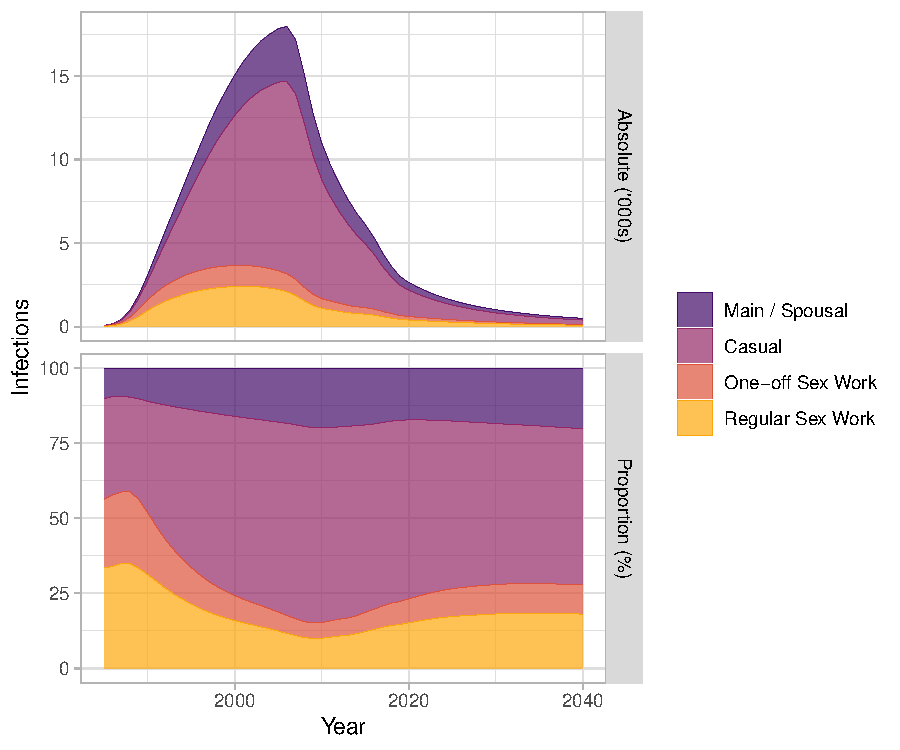
\includegraphics[width=.7\linewidth]{inf_base_part_both}
  \caption{Absolute numbers and proportions of infections
    transmitted via different modelled partnership types
    in the base case scenario}
  \label{fig:inf.part}
  \floatfoot{Median numbers of infections across all model fits are shown.}
\end{figure}
\begin{figure}[h]
  \begin{subfigure}{.5\linewidth}
    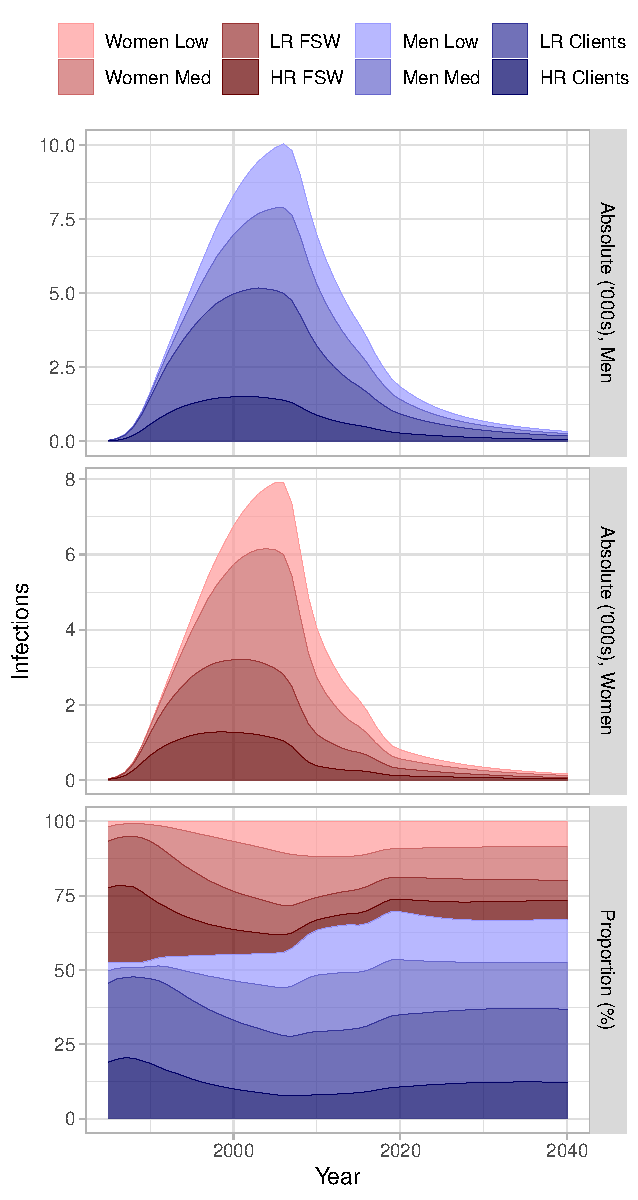
\includegraphics[width=\linewidth]{inf_base_from_both}
    \caption{Transmitted from}
    \label{fig:inf.fr}
  \end{subfigure}%
  \begin{subfigure}{.5\linewidth}
    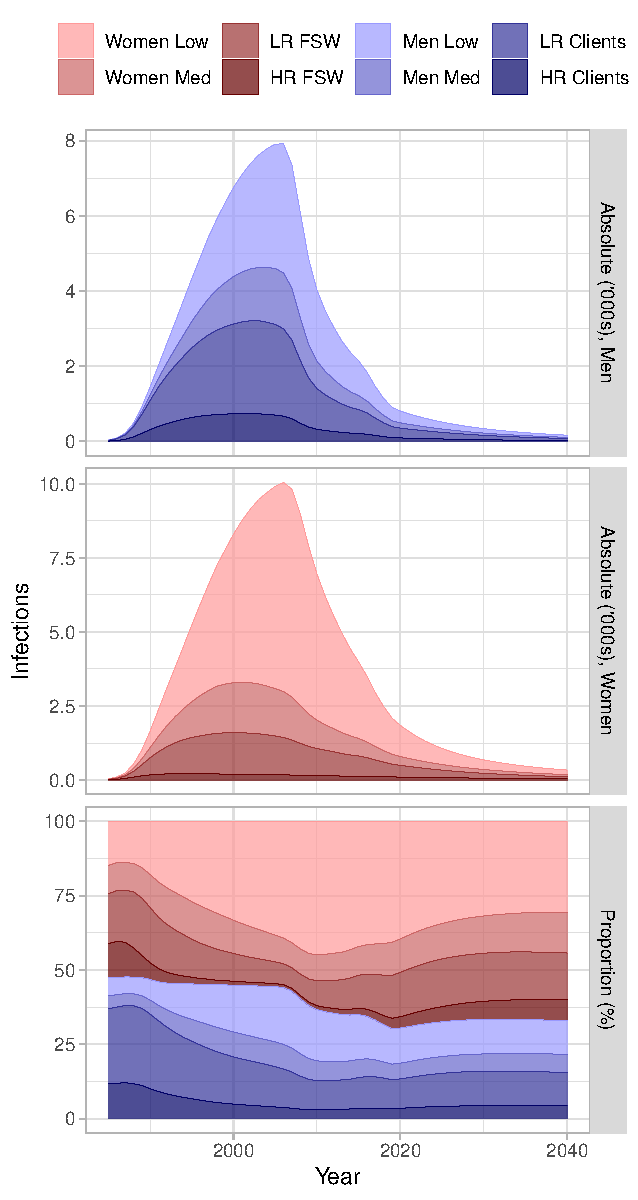
\includegraphics[width=\linewidth]{inf_base_to_both}
    \caption{Acquired among}
    \label{fig:inf.to}
  \end{subfigure}
  \caption{Absolute numbers and proportions of infections
    (\subref{fig:inf.fr}) transmitted from and (\subref{fig:inf.to}) acquired among modelled risk groups
    in the base case scenario}
  \label{fig:inf.frto}
  \floatfoot{Notation ---
    Low/LR: lower risk; Med: medium risk; HR: higher risk; FSW: female sex workers; Clients: of FSW.
    Median numbers of infections across all model fits are shown.}
\end{figure}
\begin{figure}[h]
  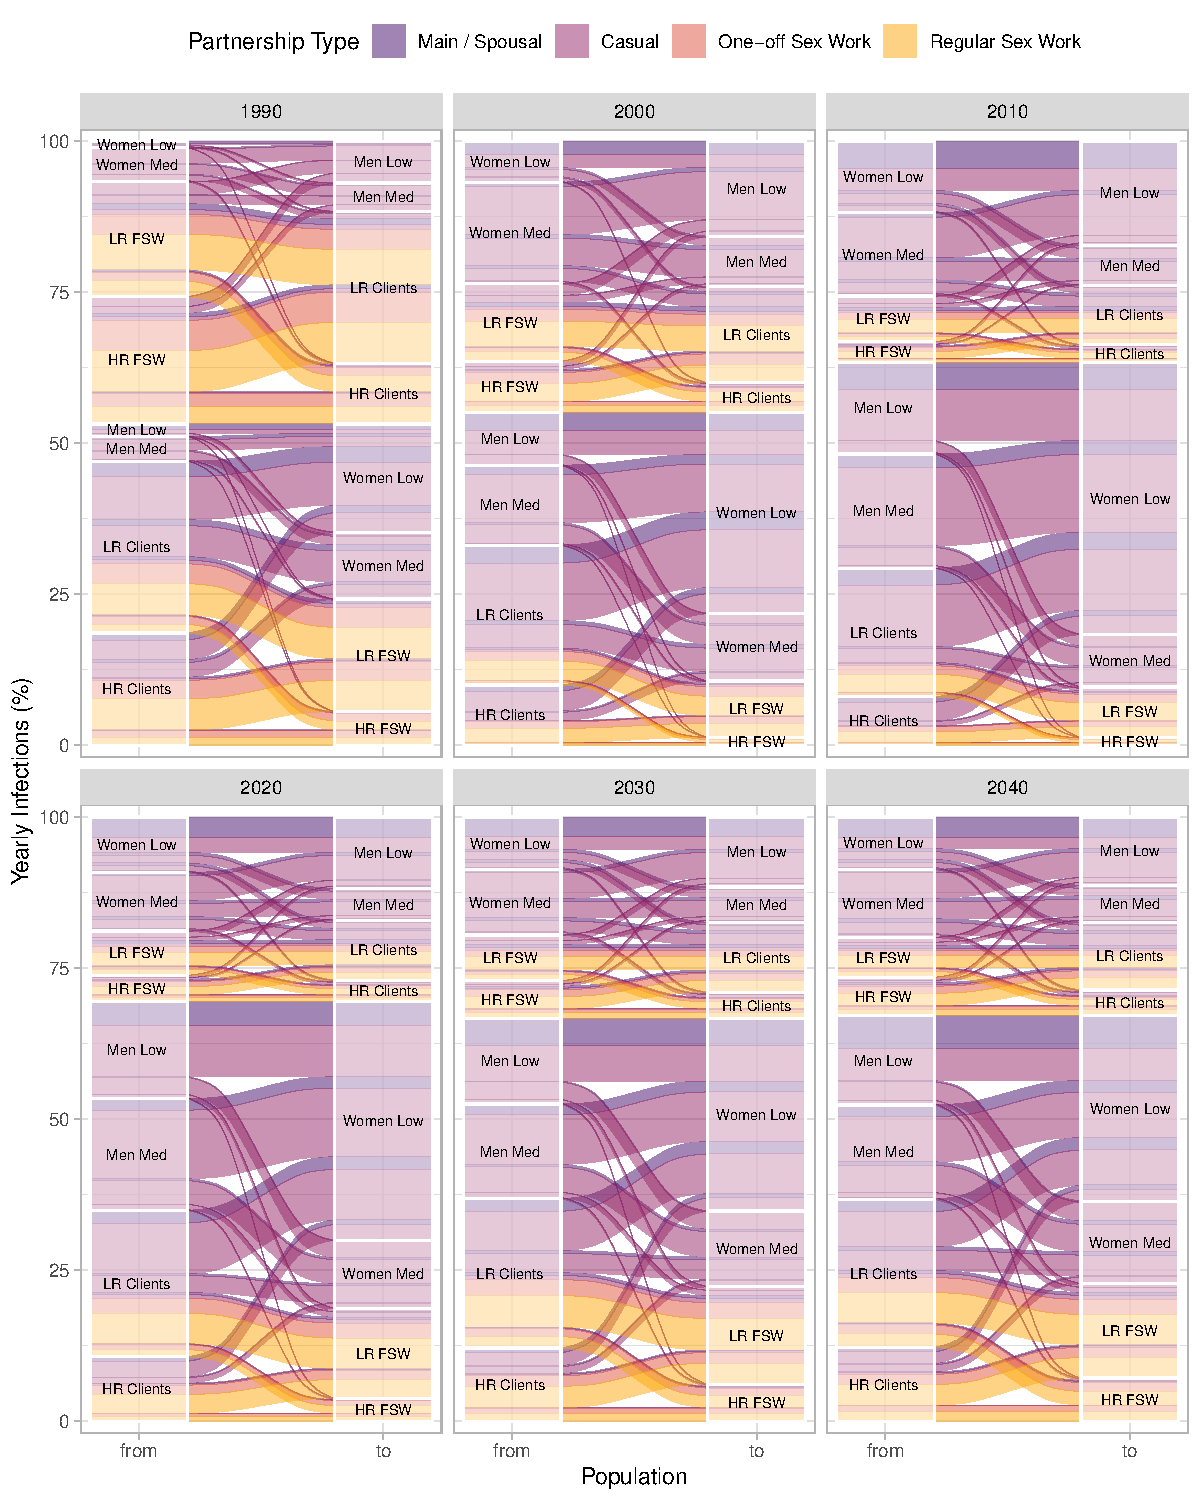
\includegraphics[width=\linewidth]{inf_base_alluvial}
  \caption{Alluvial diagram showing proportions of all yearly infections (flows)
    transmitted from (left) to (right) modelled risk groups,
    stratified by partnership type (color) and year (facets),
    in the base case scenario}
  \label{fig:inf.alluvial}
  \floatfoot{Median numbers of infections across all model fits are shown.
    An animated version of this figure is available online at
    \hreftt{github.com/mishra-lab/hiv-fsw-art}}
\end{figure}
\begin{figure}[h]
  \centering
  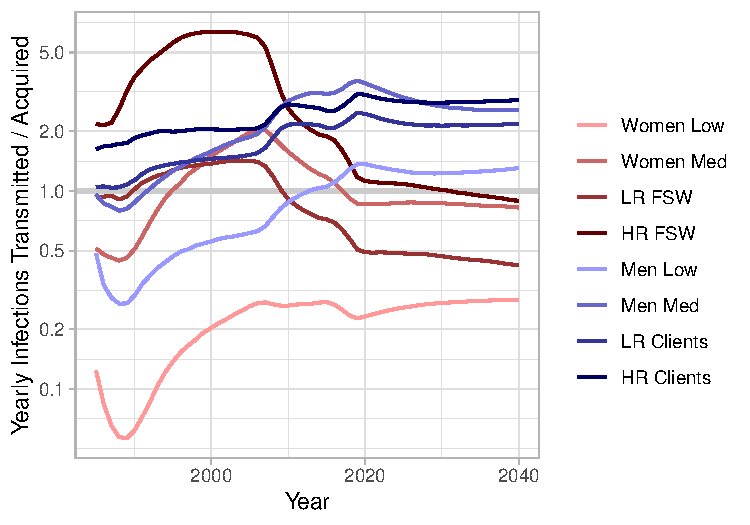
\includegraphics[width=.7\linewidth]{inf_base_ratio}
  \caption{Ratio of yearly infections transmitted from vs acquired among modelled risk groups
    in the base case scenario}
  \label{fig:inf.ratio}
  \floatfoot{Median numbers of infections across all model fits are shown.}
\end{figure}
\clearpage
%===================================================================================================
\subsection{Objective 1}\label{a:res.1}
* under construction *
%---------------------------------------------------------------------------------------------------
\subsubsection{Scenario Cascades}
Figure~\ref{fig:obj.1.cascade} illustrates \dots
\begin{figure}[h]
  \centering
  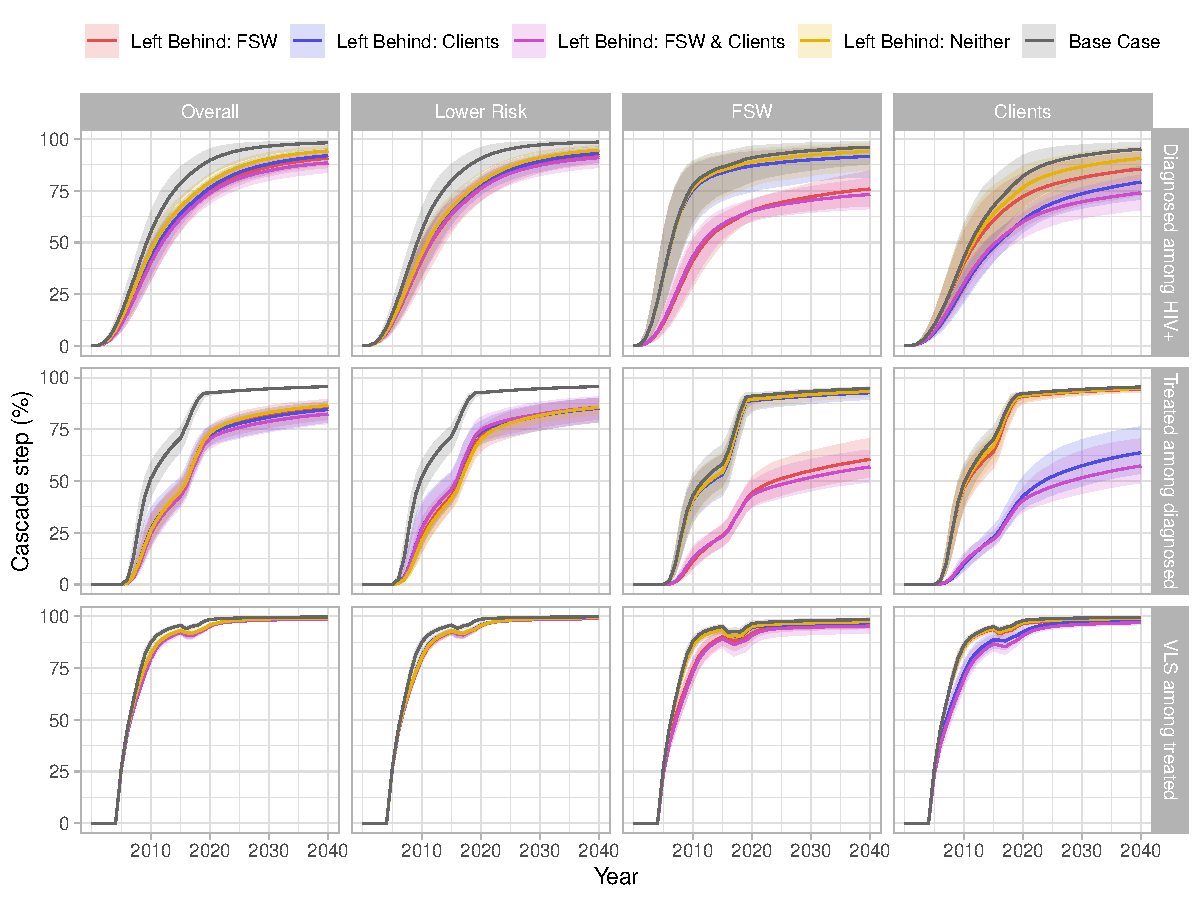
\includegraphics[width=\linewidth]{art_1_cascade}
  \caption{Cascade attainment over time in counterfactual scenarios (\casmid overall by 2020)
    vs the base case scenario (\cashigh by 2020).
    Scenarios explore reduced cascades (\caslow by 2020) among FSW, clients of FSW, both, or neither
    as part of reduced cascade overall.}
  \label{fig:obj.1.cascade}
  \floatfoot{Lines and ribbons illustrate the median and 90\% CI, respectively, for each output.}
\end{figure}
%---------------------------------------------------------------------------------------------------
\clearpage
\subsubsection{Additional Incidence}
Figure~\ref{fig:obj.1.inc} illustrates \dots
\par
Figure~\ref{fig:obj.1.inc.add} illustrates \dots
\par
\begin{figure}[h]
 \centerline{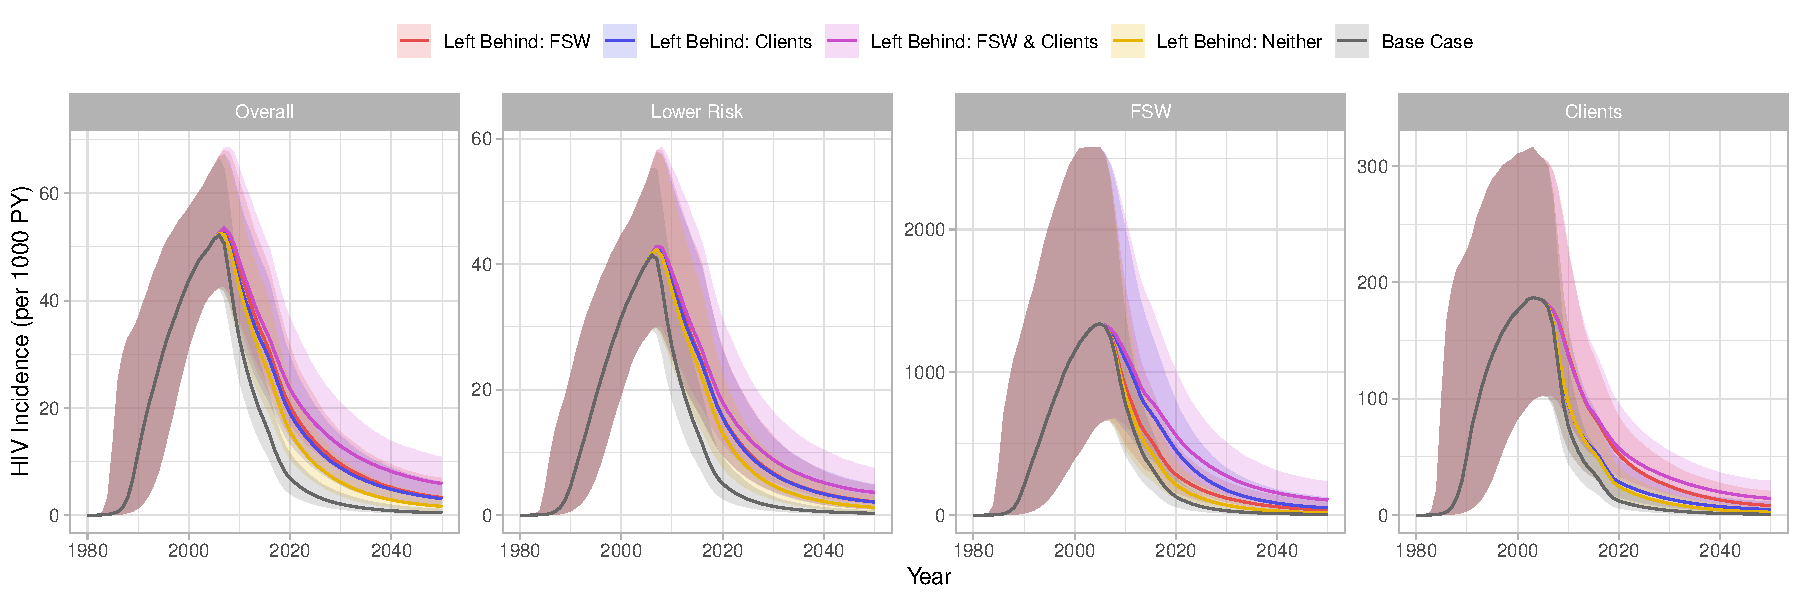
\includegraphics[width=\linewidth]{art_1_inc}}
 \caption{HIV Incidence in the base case and counterfactual scenarios}
 \label{fig:obj.1.inc}
 \floatfoot{Lines and ribbons illustrate the median and 90\% CI, respectively, for each output.}
\end{figure}
\begin{figure}[h]
  \centering
  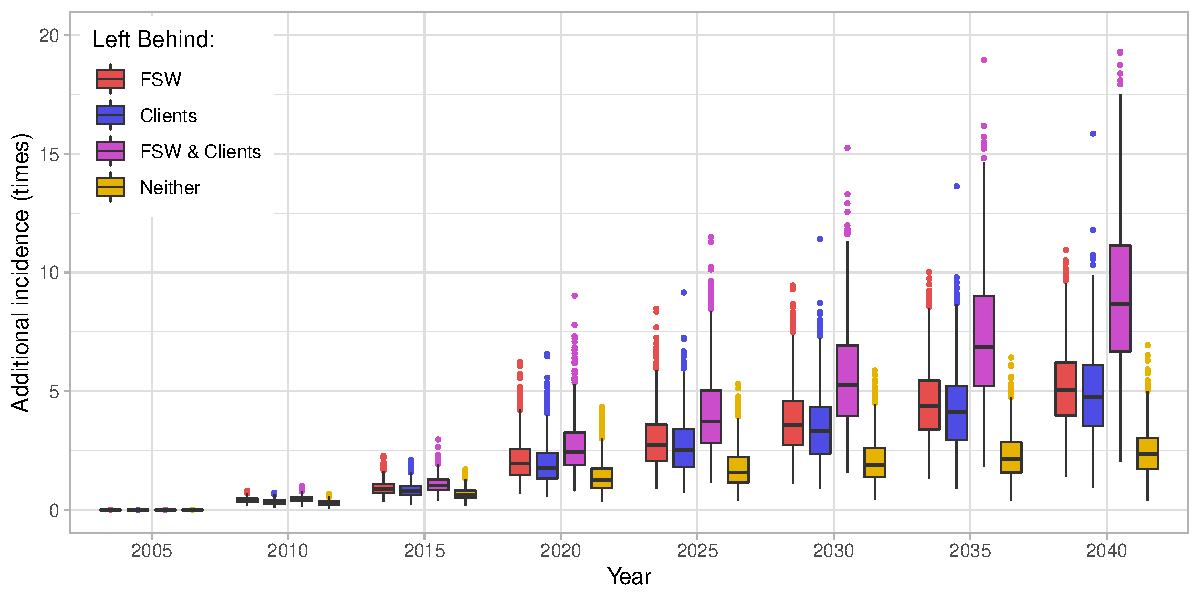
\includegraphics[width=\linewidth]{art_1_inc_add}
  \caption{Additional HIV incidence (times) in counterfactual scenarios (\casmid overall by 2020)
    vs the base case scenario (\cashigh by 2020).
    Scenarios explore reduced cascades (\caslow by 2020) among FSW, clients of FSW, both, or neither
    as part of reduced cascade overall.}
  \label{fig:obj.1.inc.add}
\end{figure}
%---------------------------------------------------------------------------------------------------
\subsubsection{Distribution of Infections}\label{a:res.1.inf}
As in \S~\ref{a:res.bc.inf}, Figure~\ref{fig:inf.diff} illustrates \dots
\clearpage\newgeometry{vscale=.85}
\begin{figure}[h]
  \begin{subfigure}{\linewidth}
    \centerline{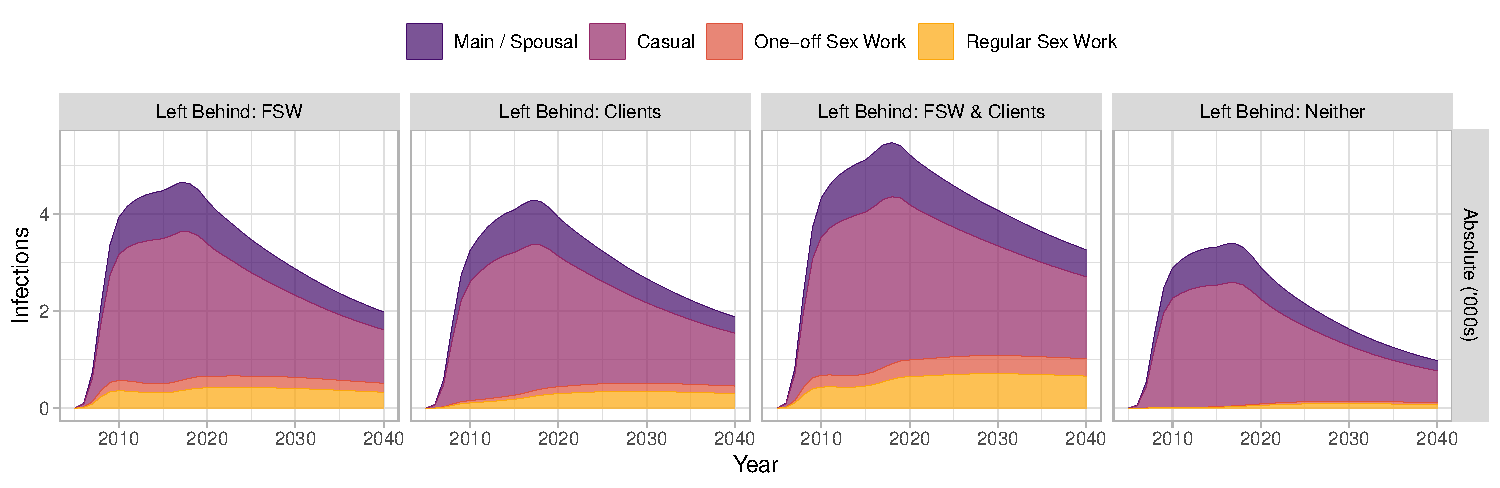
\includegraphics[width=\linewidth]{inf_diff_part_abs}}
    \caption{Partnership type}
    \label{fig:inf.diff.part}
  \end{subfigure}
  \begin{subfigure}{\linewidth}
    \centerline{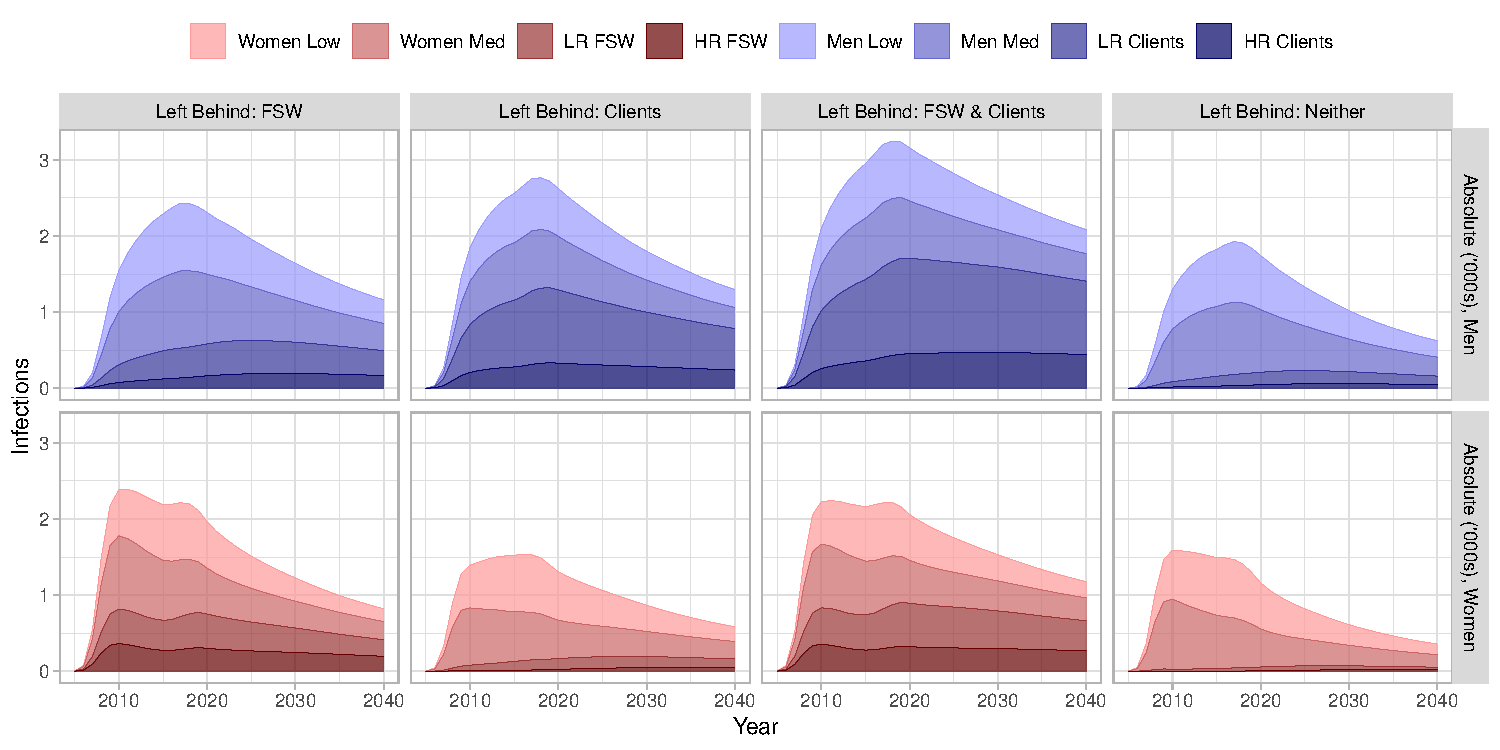
\includegraphics[width=\linewidth]{inf_diff_from_abs}}
    \caption{Transmitted from}
    \label{fig:inf.diff.from}
  \end{subfigure}
  \begin{subfigure}{\linewidth}
    \centerline{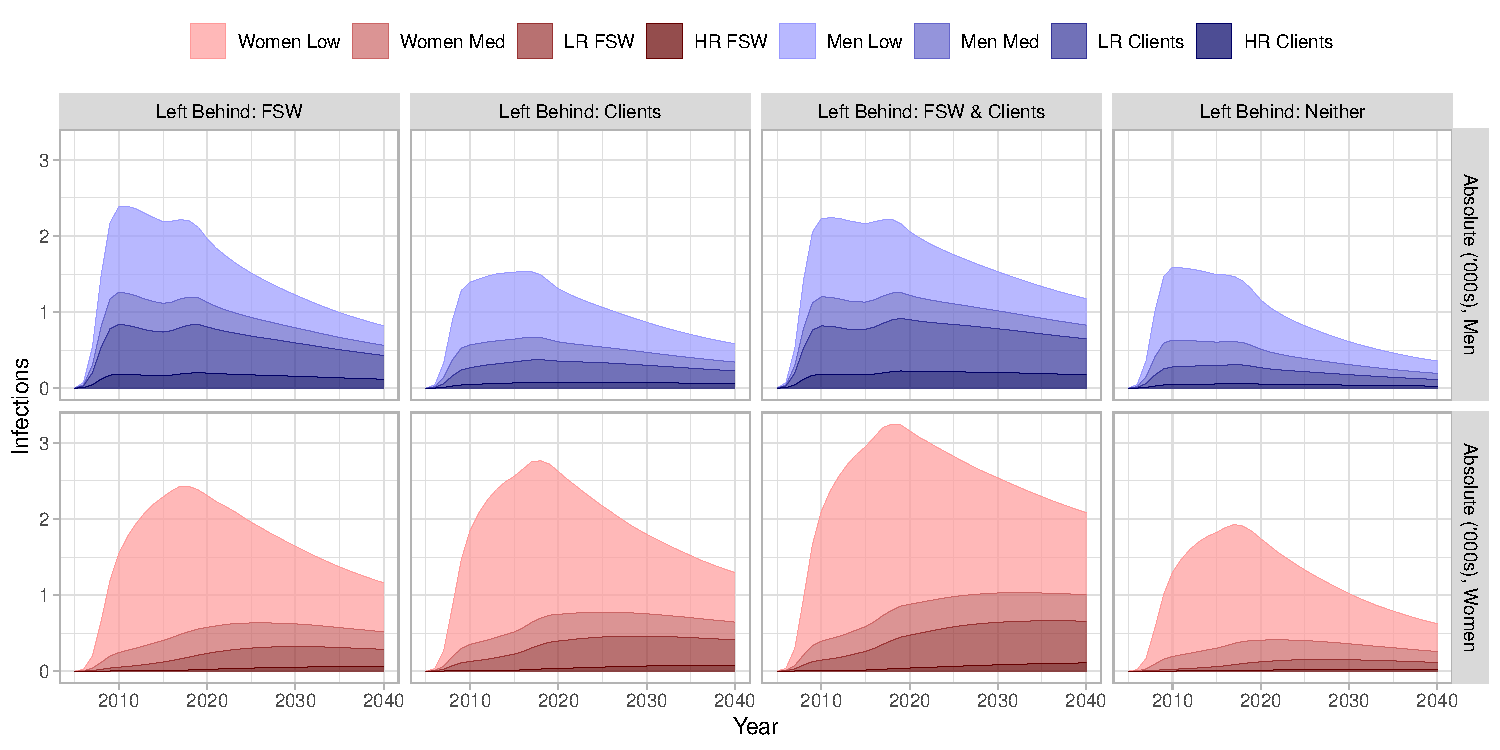
\includegraphics[width=\linewidth]{inf_diff_to_abs}}
    \caption{Acquired among}
    \label{fig:inf.diff.to}
  \end{subfigure}
  \caption{Numbers of additional infections in each counterfactual scenario vs the base case, stratified by:
    (\subref{fig:inf.diff.part}) partnership type,
    (\subref{fig:inf.diff.from}) transmitting group, and
    (\subref{fig:inf.diff.to}) acquiring group}
  \label{fig:inf.diff}
  \floatfoot{Notation ---
    Low/LR: lower risk; Med: medium risk; HR: higher risk; FSW: female sex workers; Clients: of FSW.
    Median numbers of infections across all model fits are shown.}
\end{figure}
\clearpage\restoregeometry
%===================================================================================================
\subsection{Objective 2}\label{a:res.2}
Figure~\ref{fig:obj.2.cascade} illustrates
the distribution of HIV treatment cascade attainment by 2020
in randomly sampled scenarios for Objective~\ref{obj:2}, stratified by sub-population.
Median (95\% CI) viral suppression ($VS$) among HIV+ were: % MAN TODO
43~(15,~72)\% among overall,
44~(13,~76)\% among lower risk,
45~(18,~72)\% among FSW, and
33~(9,~65)\% among clients.
\begin{figure}[h]
  \centerline{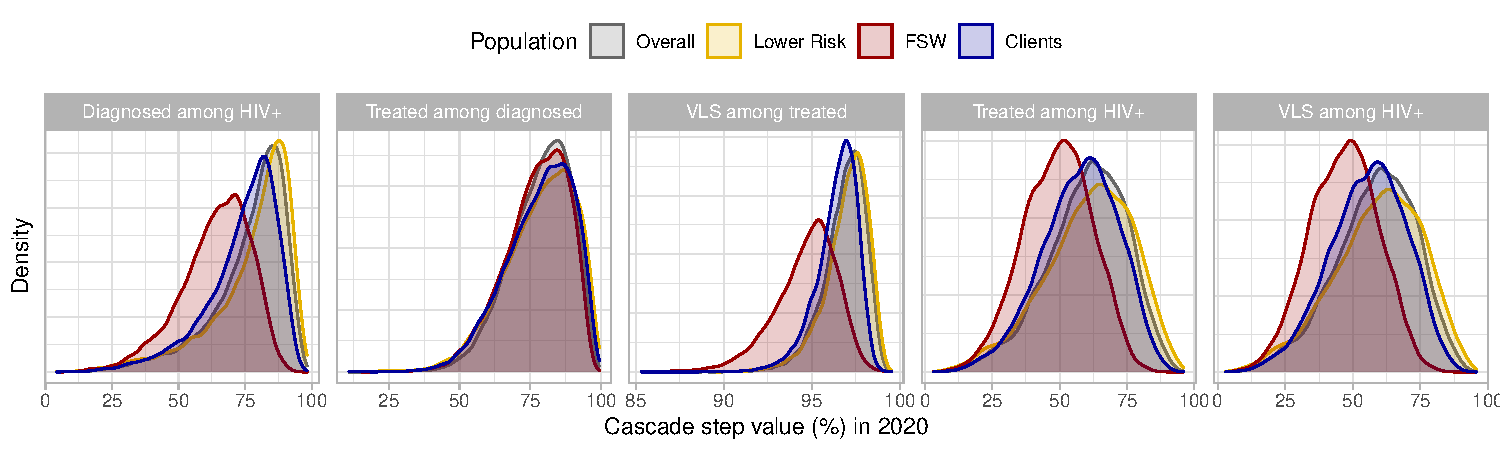
\includegraphics[width=\textwidth]{art_2_cascade}}
  \caption{Distribution of HIV treatment cascade attainment by 2020
    in randomly sampled scenarios, stratified by sub-population}
  \label{fig:obj.2.cascade}
\end{figure}
\par
Figure~\ref{fig:obj.2.inc} illustrates effects on additional incidence by 2040,
rather than cumulative additional infections.
Figure~\ref{fig:obj.2.inf.t} expands on Figure~\ref{fig:obj.2.inf}
by illustrating effects over multiple time horizons (2020, 2030, 2040).
Figure~\ref{fig:obj.2.inf.pop} expands on Figure~\ref{fig:obj.2.inf}
by illustrating effects for cumulative additional infections among different risk groups.
\begin{figure}
  \includegraphics[draft,width=\linewidth]{example-image-a}%{art_2_inc}
  \caption{Standardized effects of reduced viral suppression (d) among FSW and clients
    on \emph{additional incidence} by 2040,
    plus effect modification by epidemic conditions,
    controlling for population-overall viral suppression}
  \label{fig:obj.2.inc}
  \floatfoot{
    Points and lines show the mean and 95\% confidence interval for $\beta$ terms from Eq.~(\ref{eq:obj.2}).
    d\,X: absolute difference in viral suppression among group X versus the population overall;
    FSW: female sex workers;
    Clients: of FSW;
    LR: lower risk;
    Duration: average time spent in the risk group;
    \% Pop: relative population size;
    HIV PR: HIV prevalence ratio.
    All model variables were standardized like
    $\hat{x}_k = (x_k - \mu_{x_k}) / \sigma_{x_k}$
    to reflect the relative influence of variables.}
\end{figure}
\begin{figure}
  \includegraphics[draft,width=\linewidth]{example-image-a}%{art_2_inf_t}
  \caption{Standardized effects of reduced viral suppression (d) among FSW and clients
    on cumulative additional infections \emph{by 2020, 2030, and 2040},
    plus effect modification by epidemic conditions,
    controlling for population-overall viral suppression}
  \label{fig:obj.2.inf.t}
  \floatfoot{
    Points and lines show the mean and 95\% confidence interval for $\beta$ terms from Eq.~(\ref{eq:obj.2}).
    d\,X: absolute difference in viral suppression among group X versus the population overall;
    FSW: female sex workers;
    Clients: of FSW;
    LR: lower risk;
    Duration: average time spent in the risk group;
    \% Pop: relative population size;
    HIV PR: HIV prevalence ratio.
    All model variables were standardized like
    $\hat{x}_k = (x_k - \mu_{x_k}) / \sigma_{x_k}$
    to reflect the relative influence of variables.}
\end{figure}
\begin{figure}
  \includegraphics[draft,width=\linewidth]{example-image-a}%{art_2_inf_pop}
  \caption{Standardized effects of reduced viral suppression (d) among FSW and clients
    on cumulative additional infections \emph{among different risk groups},
    plus effect modification by epidemic conditions,
    controlling for population-overall viral suppression}
  \label{fig:obj.2.inf.pop}
  \floatfoot{
    Points and lines show the mean and 95\% confidence interval for $\beta$ terms from Eq.~(\ref{eq:obj.2}).
    d\,X: absolute difference in viral suppression among group X versus the population overall;
    FSW: female sex workers;
    Clients: of FSW;
    LR: lower risk;
    Duration: average time spent in the risk group;
    \% Pop: relative population size;
    HIV PR: HIV prevalence ratio.
    All model variables were standardized like
    $\hat{x}_k = (x_k - \mu_{x_k}) / \sigma_{x_k}$
    to reflect the relative influence of variables.}
\end{figure}



